\chapter{SINS database table}
\label{app:SINS-Database-Table}
This chapter shows a table with the different activities recorded within the SINS database. The activities are divided into the room where they were recorded.

\begin{table}[htbp]
    \centering
    \caption[SINS database recorded activities for each room]{SINS database recorded activities for each room \footnotemark}
	\label{tab:sins-database-recorded-activities}
    \begin{tabular}{l|l|c|c}
        \toprule
        \textbf{Room} & \textbf{Activity} & \textbf{Nr. ex.} & \textbf{duration (min.)} \\ 
        \midrule[1pt]
        \multirow{10}{*}{Living room} & Phone call & 22 & 8.17 $\pm$ 13.73 \\
        \cline{2-4}
        & Cooking & 19 & 16.62 $\pm$ 9.49 \\
        \cline{2-4}
        & Dish washing & 15 & 6.37 $\pm$ 1.49 \\
        \cline{2-4}
        & Eating & 19 & 7.78 $\pm$ 4.27 \\
        \cline{2-4}
        & Visit & 9 & 13.3 $\pm$ 12.11 \\
        \cline{2-4}
        & Watching TV & 13 & 155.38 $\pm$ 93.28 \\
        \cline{2-4}
        & Working & 15 & 31.24 $\pm$ 39.33 \\
        \cline{2-4}
        & Vacuum cleaning & 15 & 4.79 $\pm$ 2.14 \\
        \cline{2-4}
        & Other & 15 & 0.75 $\pm$ 0.95 \\
        \cline{2-4}
        & Absence & 15 & 66.37 $\pm$ 130.30 \\
        \midrule[1pt]
        \multirow{7}{*}{Bathroom} & Drying with towel & 10 & 1.67 $\pm$ 0.28 \\
        \cline{2-4}
        & Shaving & 13 & 1.91 $\pm$ 1.46 \\
        \cline{2-4}
        & Showering & 10 & 6.11 $\pm$ 2.38 \\
        \cline{2-4}
        & Tooth brushing & 19 & 1.41 $\pm$ 0.25 \\
        \cline{2-4}
        & Vacuum cleaning & 9 & 0.87 $\pm$ 0.59 \\
        \cline{2-4}
        & Other & 75 & 0.42 $\pm$ 0.4 \\
        \cline{2-4}
        & Absence & 35 & 248.56 $\pm$ 263.62 \\
        \midrule[1pt]
        \multirow{3}{*}{Hall} & Vacuum cleaning & 9 & 3.31 $\pm$ 1.11 \\
        \cline{2-4}
        & Other & 164 & 0.36 $\pm$ 0.22 \\
        \cline{2-4}
        & Absence & 175 & 50.17 $\pm$ 102.52 \\
        \midrule[1pt]
        \multirow{3}{*}{Toilet} & Toilet visit & 21 & 4.74 $\pm$ 3.24 \\
        \cline{2-4}
        & Vacuum cleaning & 7 & 0.53 $\pm$ 0.07 \\
        \cline{2-4}
        & Absence & 31 & 282.75 $\pm$ 263.19 \\
        \midrule[1pt]
        \multirow{5}{*}{Bedroom} & Dressing & 28 & 1.53 $\pm$ 1.10 \\
        \cline{2-4}
        & Sleeping & 7 & 348.43 $\pm$ 130.73 \\
        \cline{2-4}
        & Vacuum cleaning & 7 & 1.04 $\pm$ 0.27 \\
        \cline{2-4}
        & Other & 22 & 0.27 $\pm$ 0.23 \\
        \cline{2-4}
        & Absence & 22 & 122.28 $\pm$ 157.43 \\
        \bottomrule
    \end{tabular}
\end{table}
\footnotetext{\fullcite{dekkers_sins_2017}}

\chapter{Milestone reports}
\label{app:Milestone-Reports}
This chapter lists the individual milestone reports. These should provide information on the status of the project during the realisation. For every completed milestone, a report was written before the next phase could be started. The table \fullref{tab:Milestones} shows the milestones within the thesis as well as the corresponding dates when the milestone and the phase will be completed and reviewed. The milestones are also shown in the whole project plan in \fullref{fig:Project-Plan}.

\section{Milestone report M1 from the 15.03.2020}
In the first phase of the project, the main goal was to research the subjects used for the thesis. Within phase, the project also had to be initialised and started. More precisely, the project structure and documentation also had to be defined. The goal was also to finish the first chapter of the thesis \fullref{ch:Related-Work} along with the research.

\begin{table}[htbp]
    \centering
    \caption{Work carried out milestone M1 (15.03.2020)}
	\label{tab:Work-Carried-Out-M1}
    \begin{tabular}{p{.70\textwidth} | p{.20\textwidth}}
        \toprule
        \textbf{Task} & \textbf{Status} \\ 
        \midrule[1pt]
        Research: Dataset & finished \\
        \hline
        Research: Audio processing & finished \\
        \hline
        Research: Triplet Loss & finished \\
        \hline
        Research: Tile2Vec & finished \\
        \hline
        Research: Evaluate research & finished \\
        \hline
        Realisation: Project setup & started \\
        \hline
        Realisation: Input pipeline & started \\
        \bottomrule
    \end{tabular}
\end{table}

\subsection{What work was carried out in the last reporting period}
The tasks carried out within this period are shown in the table \fullref{tab:Work-Carried-Out-M1}, along with the status of the task at the time of the milestone review. A detailed report on the entire tasks carried out within the period is shown in the work journal \ref{tab:Work-Journal}. To reach the goal of simultaneously finishing the chapter \ref{ch:Related-Work} with the research, each researched topic was documented right away. 
\subsection{State of progress}
The current milestone was successfully reached since all the planned tasks could be finished. The phase was finished too early so that the next period could already be started, the realisation phase. 

\subsection{Top three risks including planned measures}
\begin{enumerate}
    \setlength\itemsep{0em}
    \item Formulas related work wrong, will be checked by Daniel Pfäffli
    \item Topics missing in related work, will be checked by Daniel Pfäffli
    \item Input pipeline structure, will be discussed at the next meeting
\end{enumerate}

\section{Milestone report M2 from the 29.03.2020}
In the second milestone of the project, the main goal was to finish the whole project setup. The project repository had to be set up, the input pipeline was created for the dataset, and the default model architecture was created. The purpose was that after this milestone, the project is at a certain point, that the implementation of specific architectures is fast enough to experiment with different ones.

\begin{table}[htbp]
    \centering
    \caption{Work carried out milestone M2 (29.03.2020)}
	\label{tab:Work-Carried-Out-M2}
    \begin{tabular}{p{.70\textwidth} | p{.20\textwidth}}
        \toprule
        \textbf{Task} & \textbf{Status} \\ 
        \midrule[1pt]
        Realisation: Project setup & finished \\
        \hline
        Realisation: Input pipeline & finished \\
        \hline
        Realisation: Default architecture & finished \\
        \hline
        Realisation: Evaluation Workflow & midway \\
        \hline
        Realisation: Unit tests & midway \\
        \bottomrule
    \end{tabular}
\end{table}

\subsection{What work was carried out in the last reporting period}
The tasks carried out within this period are shown in the table \fullref{tab:Work-Carried-Out-M2}, along with the status of the task at the time of the milestone review. A detailed report on the entire tasks carried out within the period is shown in the work journal \ref{tab:Work-Journal}. Two tasks were not completed within the period, which was now prioritised in the next phase and will get completed first. The milestone could not be completed because to little time was planned for tasks like \flqq input pipeline\frqq or \flqq evaluation workflow\frqq. The evaluation workflow was completed except for the classifier, to evaluate the architecture in relation to the other models in the DCASE Challenge. Unit tests were not written for all the created models but will be right away at the start of the next milestone.

\subsection{State of progress}
The current milestone was not reached since two tasks could not be finished entirely. The uncompleted tasks were prioritised and were moved to the next phase of the project.

\subsection{Top three risks including planned measures}
\begin{enumerate}
    \setlength\itemsep{0em}
    \item GPU caching / file deletion problem, will be discussed at the next meeting
    \item Classifier architecture, will be discussed at the next meeting
    \item Unit tests for models, will be discussed at the next meeting 
\end{enumerate}

\section{Milestone report M3 from the 12.04.2020}
The third milestone aimed to finalise the realisation. The idea of unsupervised triplet loss had to be implemented, like the one from Tile2Vec for both datasets. Furthermore, an easy to use architecture for the experiments had to be developed. Thus the experiments should be conducted relatively simple. The main goal is to provide an architecture which is reliable, arbitrarily expandable and repeatable. All of these points are essential for conducting successful experiments.

\begin{table}[htbp]
    \centering
    \caption{Work carried out milestone M3 (12.04.2020)}
	\label{tab:Work-Carried-Out-M3}
    \begin{tabular}{p{.70\textwidth} | p{.20\textwidth}}
        \toprule
        \textbf{Task} & \textbf{Status} \\ 
        \midrule[1pt]
        Realisation: Evaluation Workflow & finished \\
        \hline
        Realisation: Unit tests & finished \\
        \hline
        Realisation: Tile2Vec implementation & finished \\
        \hline
        Realisation: Architecture for experiments & finished \\
        \hline
        Experiments: Conduct experiments & started \\
        \bottomrule
    \end{tabular}
\end{table}

\subsection{What work was carried out in the last reporting period}
The tasks carried out within this period are shown in the table \fullref{tab:Work-Carried-Out-M3}, along with the status of the task at the time of the milestone review. A detailed report on the entire tasks carried out within the period is shown in the work journal \ref{tab:Work-Journal}. Two tasks were not completed during the last phase and were completed at the start of this phase by prioritising them. Both of the other tasks which were planned to complete during this phase were completed.

\subsection{State of progress}
The current milestone was successfully reached since all the planned tasks could be finished. The phase was finished too early so that the next period could already be started, the experiment phase. 

\subsection{Top three risks including planned measures}
\begin{enumerate}
    \setlength\itemsep{0em}
    \item Review evaluation workflow, will be discussed at the next meeting
    \item Review of study doc, will be discussed at the next meeting
    \item Review of test concept, will be discussed at the next meeting 
\end{enumerate}

\section{Milestone report M5 from the 03.05.2020}
The last milestone before the thesis submission is the M5, which concludes the experiment phase. In the experiment phase, all of the experiments are conducted and validated. For each experiment, a separate study doc is written, which describes the experiments in more detail, and can be found in \ref{app:Study-Doc}. Within this phase, a lot of different experiments are conducted to find the optimal parameters for the problem definition. In this phase, the codebase will be adjusted if problems are found or if new ideas need to be implemented. The purpose of these adjustments is always to improve the performance of the models.
\begin{table}[htbp]
    \centering
    \caption{Work carried out milestone M5 (03.05.2020)}
	\label{tab:Work-Carried-Out-M5}
    \begin{tabular}{p{.70\textwidth} | p{.20\textwidth}}
        \toprule
        \textbf{Task} & \textbf{Status} \\ 
        \midrule[1pt]
        Experiments: Conduct experiments & midway \\
        \hline
        Experiments: Validate experiments & midway \\
        \bottomrule
    \end{tabular}
\end{table}

\subsection{What work was carried out in the last reporting period}
The tasks carried out within this period are shown in the table \fullref{tab:Work-Carried-Out-M5}, along with the status of the task at the time of the milestone review. A detailed report on the entire tasks carried out within the period is shown in the work journal \ref{tab:Work-Journal}. Both of the tasks were not completed during the phase. That the tasks were not completed is because there were more experiments to conduct than intentionally thought. There was also the problem that some of the experiments took a long time to be conducted due to the lack of additional computing resources. Both tasks will be prioritised and completed in the next phase. 

\subsection{State of progress}
The current milestone was not reached since two tasks could not be finished entirely. The uncompleted tasks were prioritised and were moved to the next phase of the project.

\subsection{Top three risks including planned measures}
\begin{enumerate}
    \setlength\itemsep{0em}
    \item Not enough time to conduct all experiments; therefore the buffer phase will be used to conduct additional experiments
    \item Not enough time to conduct all experiments; therefore additional computing power will be rented at \texttt{vast.ai}
    \item Not enough experience with the hyperparameters; therefore will be discussed within the next meeting
\end{enumerate}

\clearpage
\landscapevalues

\chapter{Test concept}
\label{app:Test-Concept}
This chapter of the appendix contains detailed information about the manual tests conducted in the project to test each component thoroughly. For each manually conducted test case the steps, the status, the expected result and the actual result is given. The automated tests can be found in the \texttt{test} directory of the source code repository.

\begin{longtable}{p{.15\textwidth} | p{.40\textwidth} | p{.05\textwidth} | p{.15\textwidth} | p{.15\textwidth}}
        \caption{Test concept of the manual conducted tests}
	    \label{tab:Test-Concept} \\
        \toprule
        \textbf{Test case} & \textbf{Steps} & \textbf{Status} & \textbf{Expected result} & \textbf{Actual result} \\ 
    \midrule[1pt]
        Embedding models successfully train & 
        \begin{minipage}{3.8in}
        \vskip 4pt
        For each of the embedding models in the project:
        \begin{enumerate}
        \setlength\itemsep{0em}
        \item choose the embedding model to train
        \item train the model for ten epochs on the DCASE dataset
        \item check if the model started to converge during the training, by checking if the triplet loss value decreases
        \end{enumerate}
        \vskip 4pt
        \end{minipage} & \cellcolor{green!30!white}passed & models converge & all of the models converged during the training \\
    \hline
        Classifier models successfully train & 
        \begin{minipage}{3.8in}
        \vskip 4pt
        For each of the classifier models in the project:
        \begin{enumerate}
        \setlength\itemsep{0em}
        \item choose a trained embedding model to embed the segments into the embedding space
        \item choose the classifier model to train
        \item train the classifier for ten epochs on the DCASE dataset
        \item for each of the segments in the dataset, embed and then feed them to the classifier
        \item check if the model started to converge during the training, by checking if the sparse categorical cross-entropy loss decreases 
        \end{enumerate}
        \vskip 4pt
        \end{minipage} & \cellcolor{green!30!white}passed & classifiers converge & all of the classifiers converged during the training \\
    \hline
        Training process works & 
        \begin{minipage}{3.8in}
        \vskip 4pt
        \begin{enumerate}
        \setlength\itemsep{0em}
        \item choose a random embedding model, optimally not a very computing intensive one
        \item train the model for ten epochs on the DCASE dataset
        \item check if after ten epochs the training terminates
        \item check if there were no errors during the training, for example because of the input pipeline
        \item check if all of the metrics are correctly displayed on the Tensorboard
        \item check if all of the metrics seem reasonable, no extremely low or high values after a few epochs
        \item check if the model is successfully saved at the end of each epoch
        \end{enumerate}
        \vskip 4pt
        \end{minipage} & \cellcolor{green!30!white}passed & training process works & all of the checks were successfully and therefore the training process works \\
    \hline
        Training process stopped and started again & 
        \begin{minipage}{3.8in}
        \vskip 4pt
        \begin{enumerate}
        \setlength\itemsep{0em}
        \item choose a random embedding model, optimally not a very computing intensive one
        \item train the model for ten epochs on the DCASE dataset
        \item after five epochs, stop the training procedure
        \item start the training procedure again for five epochs with the same model, by changing the params in the \texttt{params.json} file
        \item check if the model was successfully loaded
        \item check if the model was trained from the fifth epoch again and not from scratch
        \item check if there were no errors during the training, for example because of the input pipeline
        \item check if the metrics show that the model was stopped during the training
        \item check if the model is successfully saved
        \end{enumerate}
        \vskip 4pt
        \end{minipage} & \cellcolor{green!30!white}passed & training process loads models correctly & all of the checks were successfully and therefore the training process for loading already trained models works, the metrics further show a continuous graph even if the training is stopped and than started again \\
    \bottomrule
\end{longtable}

\clearpage
\defaultpagestyle

\chapter{Study doc}
\label{app:Study-Doc}
This chapter contains all of the study docs from the conducted experiments, they include detailed information about each one of the experiments as well as the conclusion out of each.

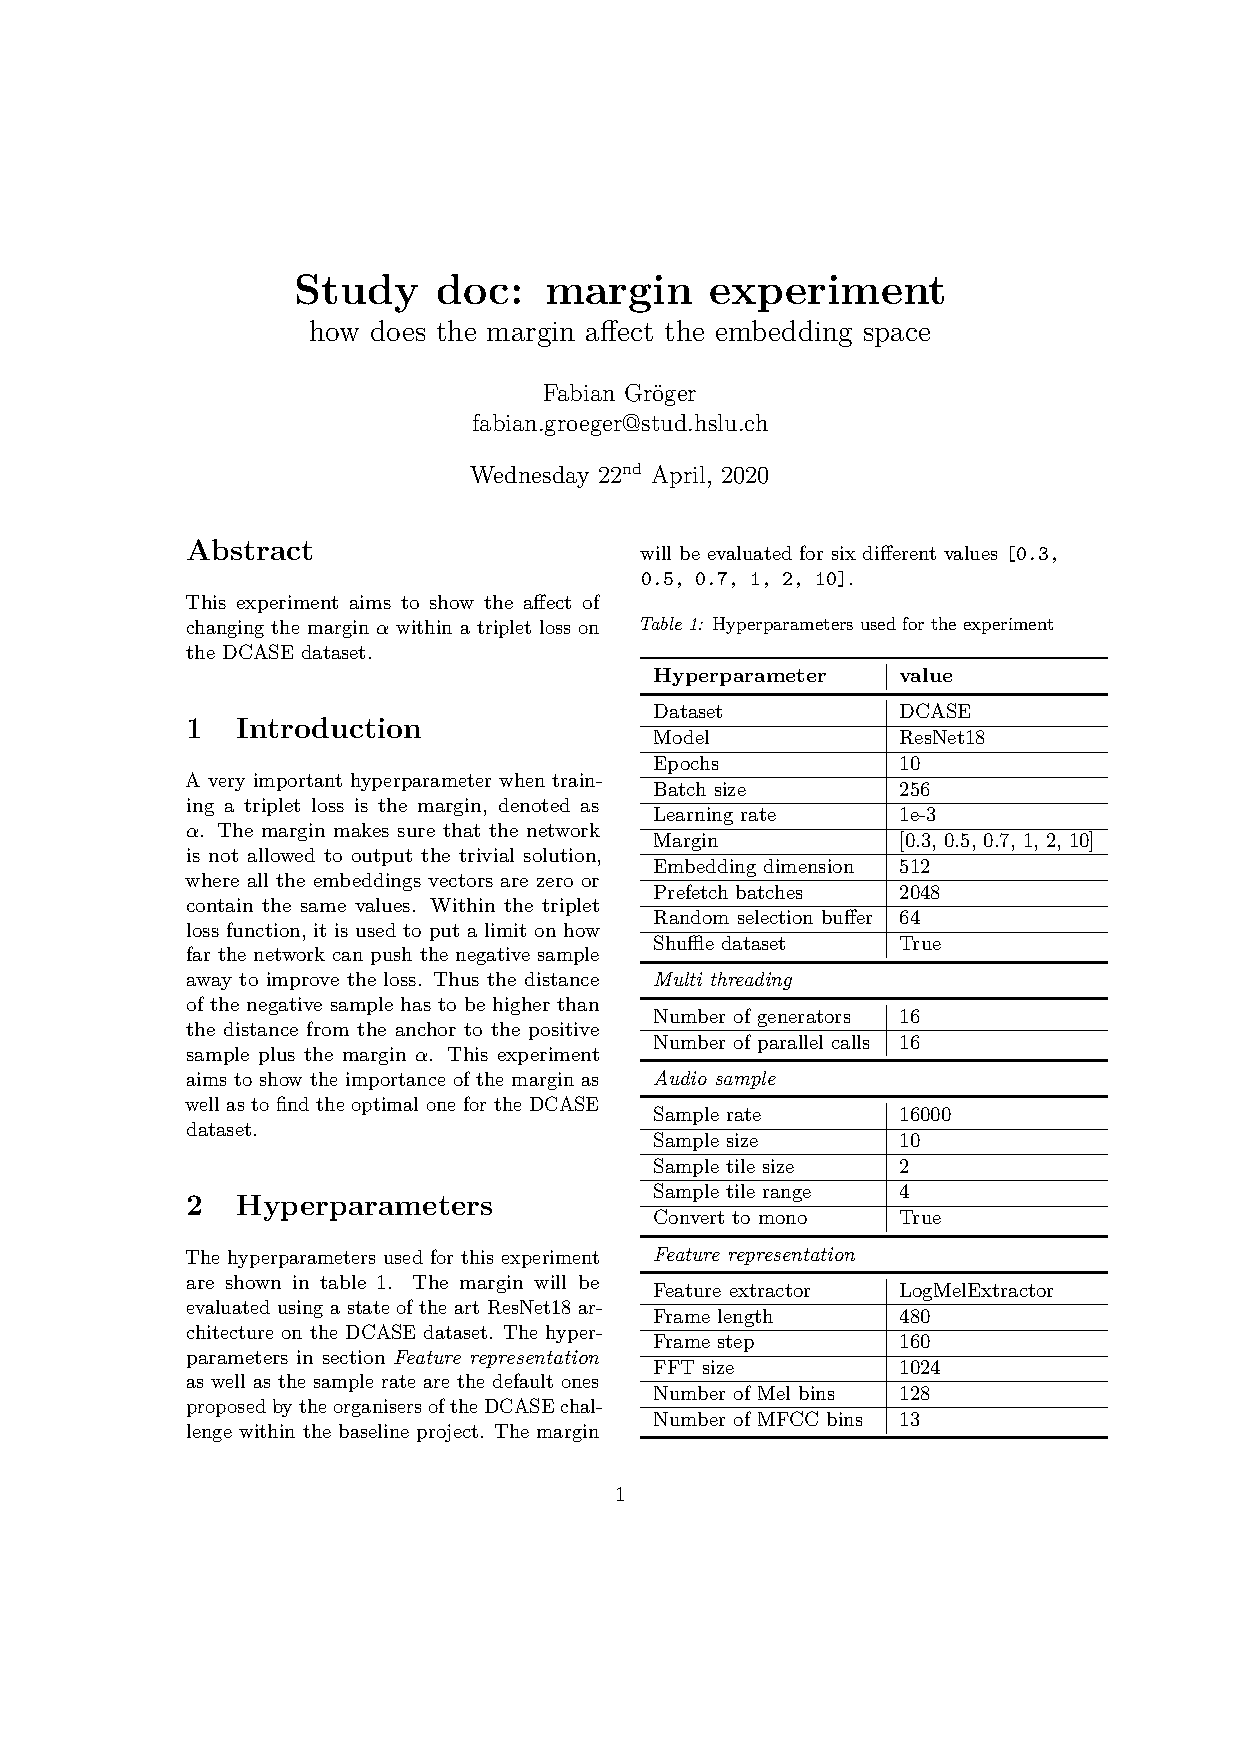
\includepdf[scale=1.0, pages=1-]{study-doc/experiment_margin/Study_Doc_Margin.pdf}

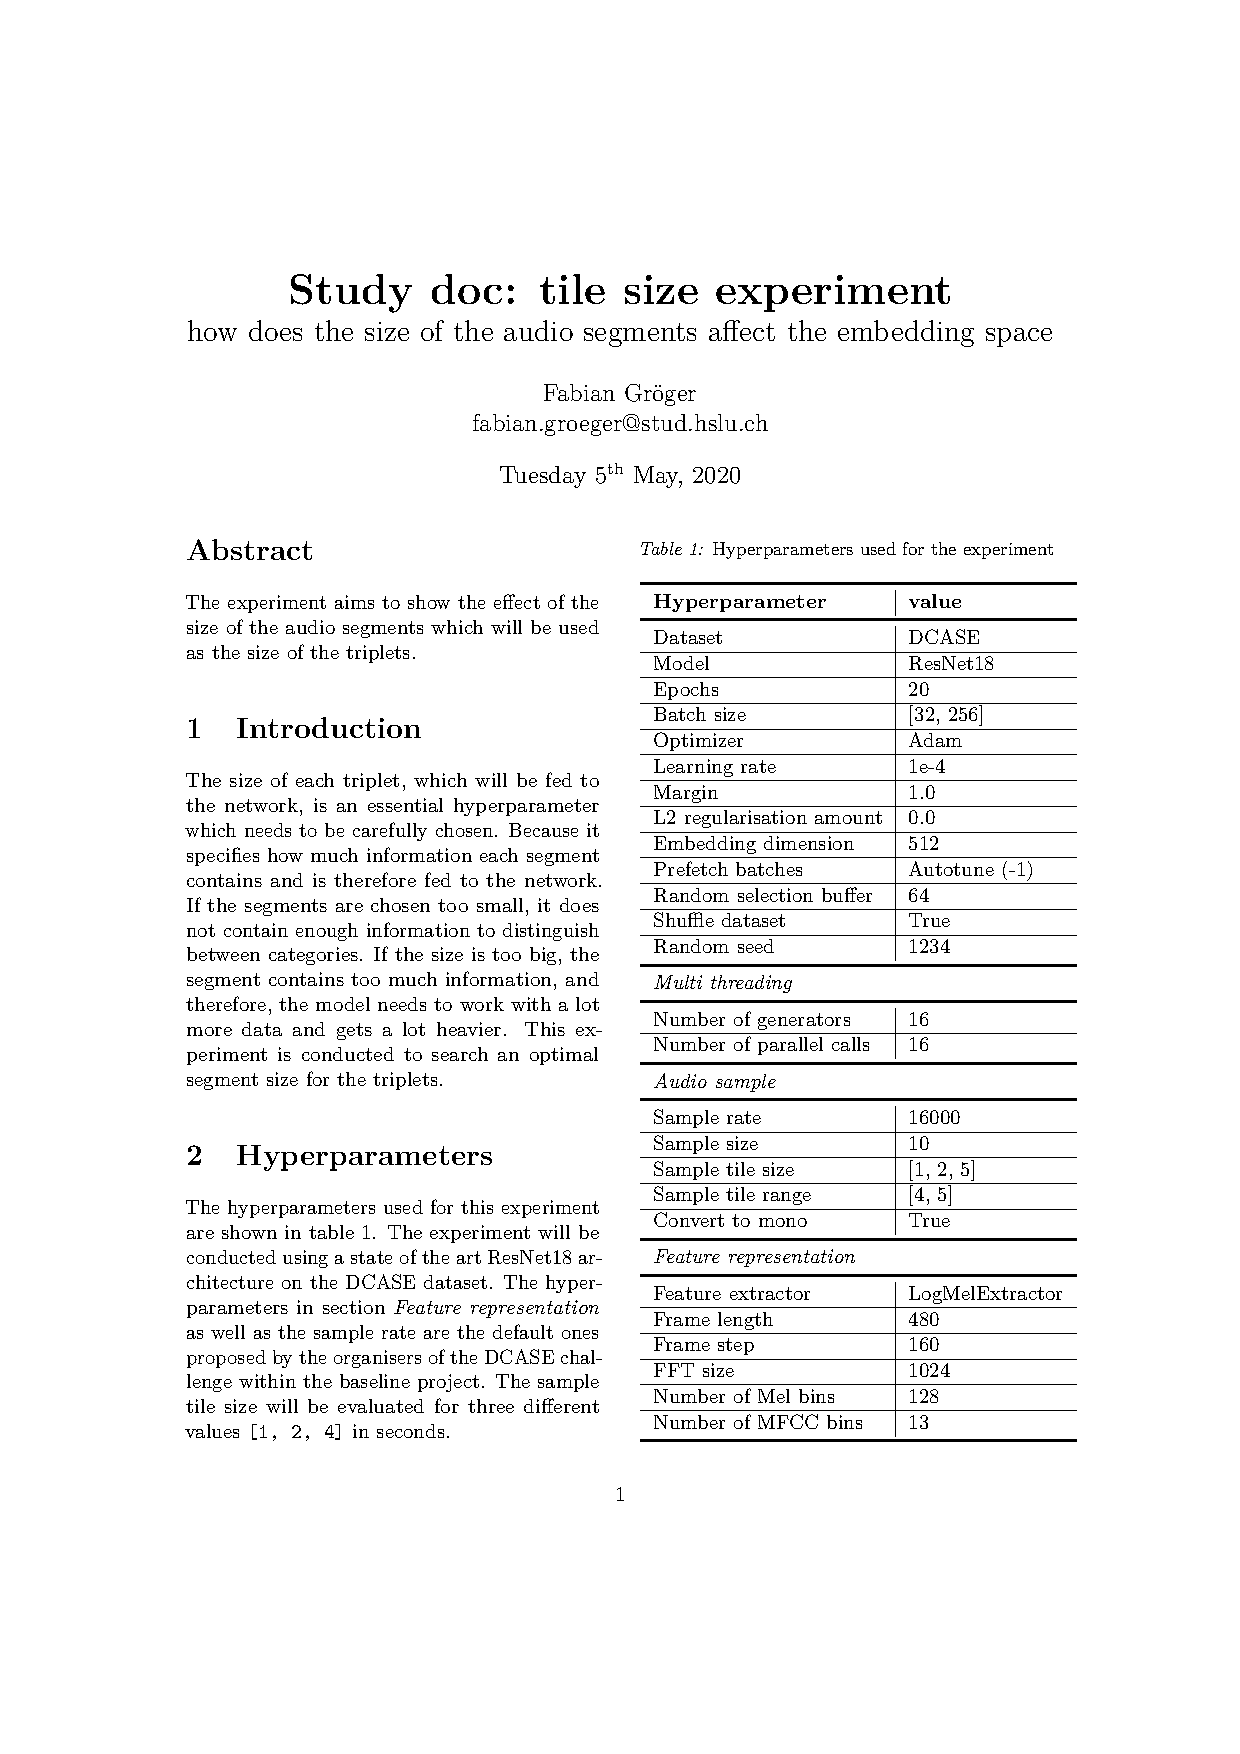
\includepdf[scale=1.0, pages=1-]{study-doc/experiment_tile_size/Study_Doc_tile_size.pdf}

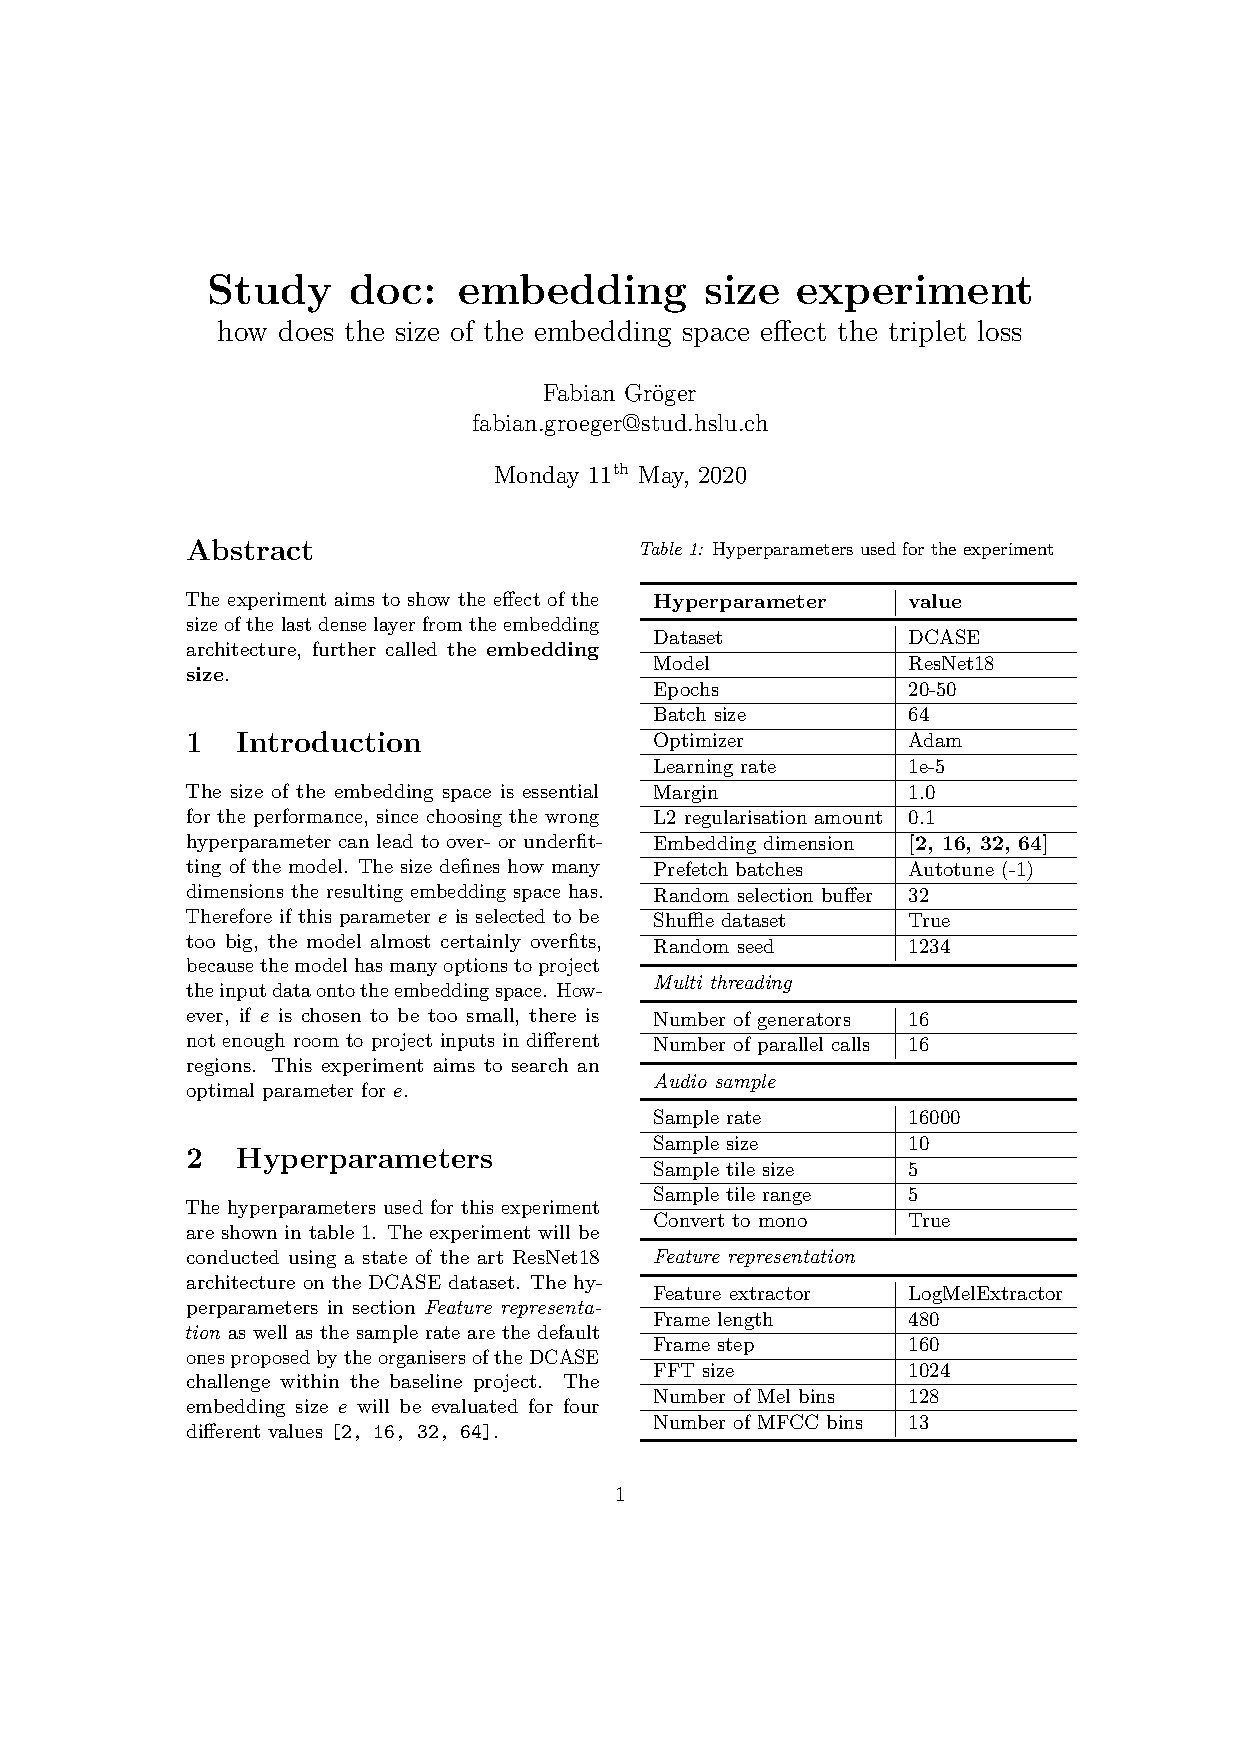
\includepdf[scale=1.0, pages=1-]{study-doc/experiment_embedding_size/Study_Doc_embedding_size.pdf}

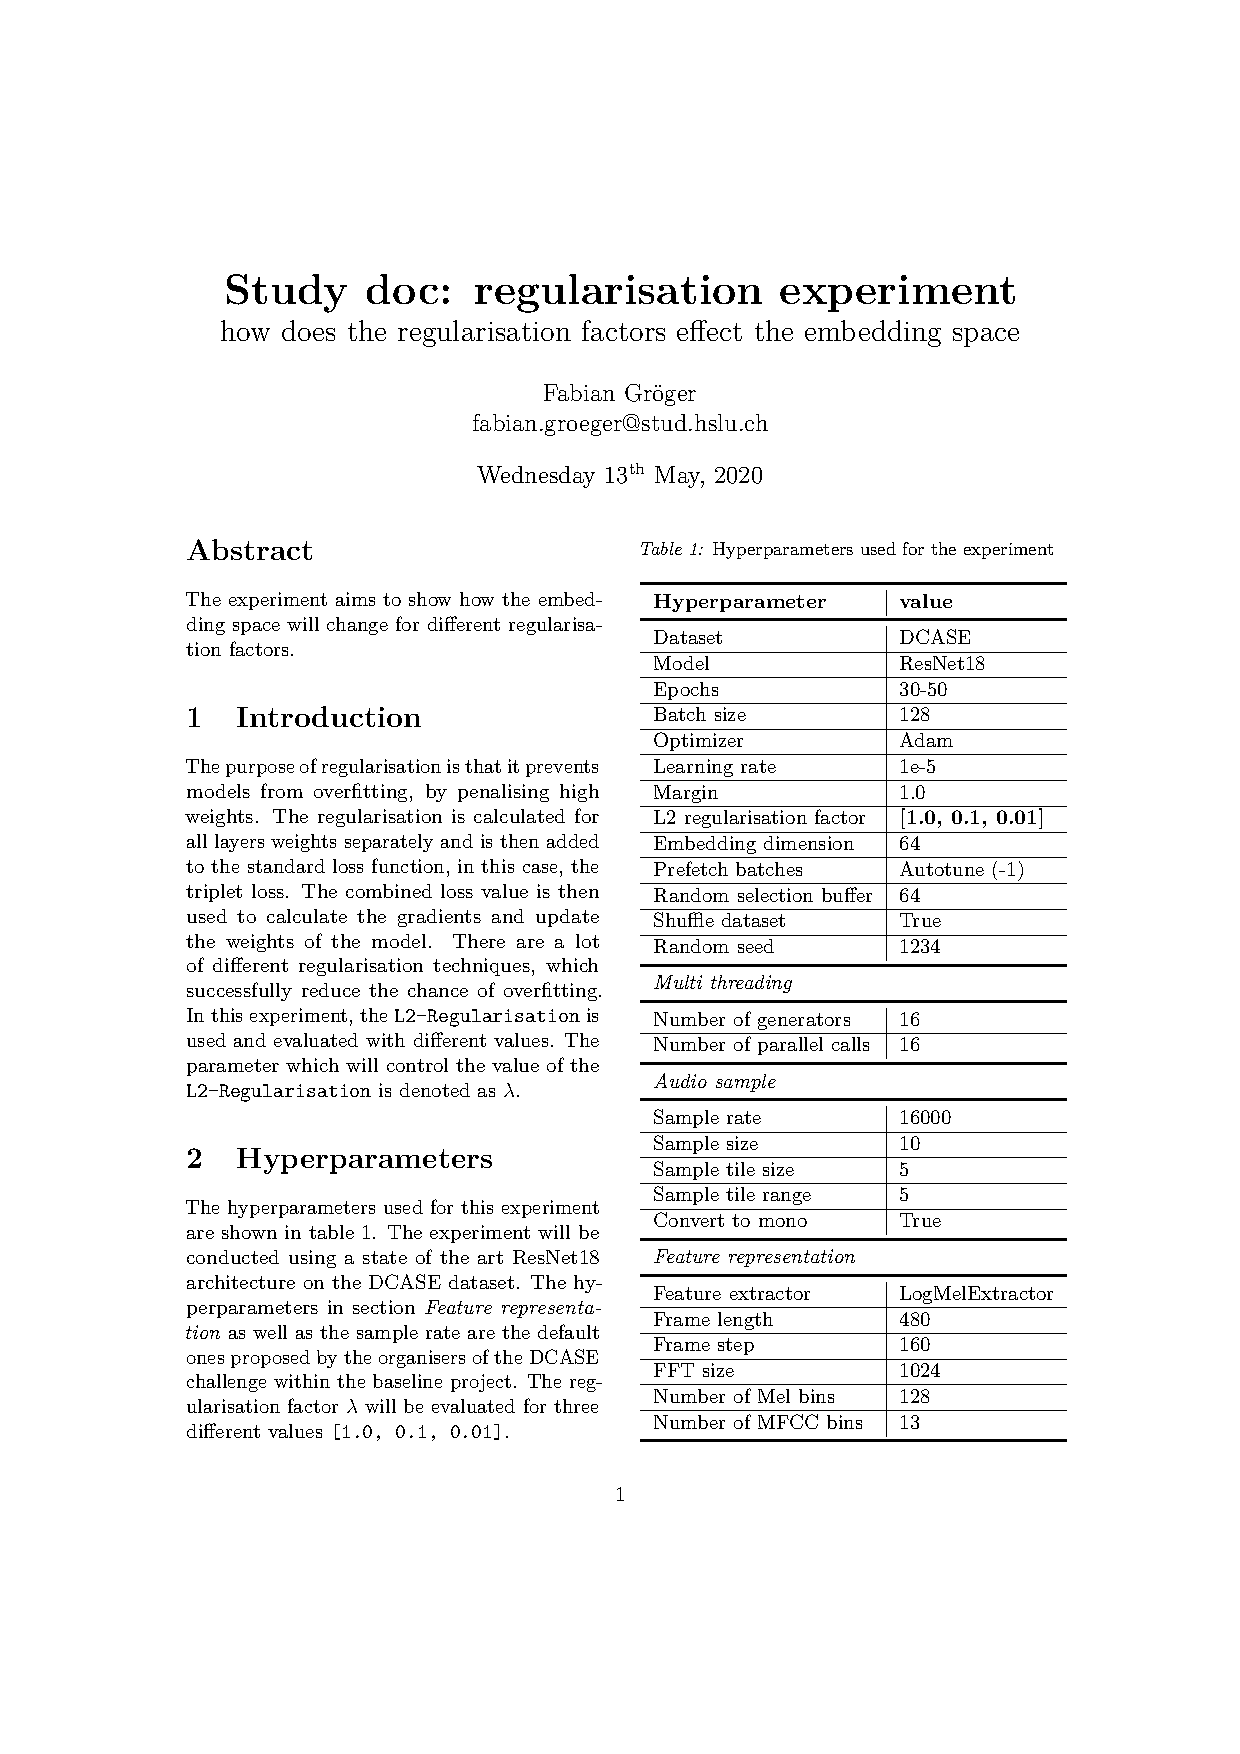
\includepdf[scale=1.0, pages=1-]{study-doc/experiment_regularisation/Study_Doc_regularisation.pdf}

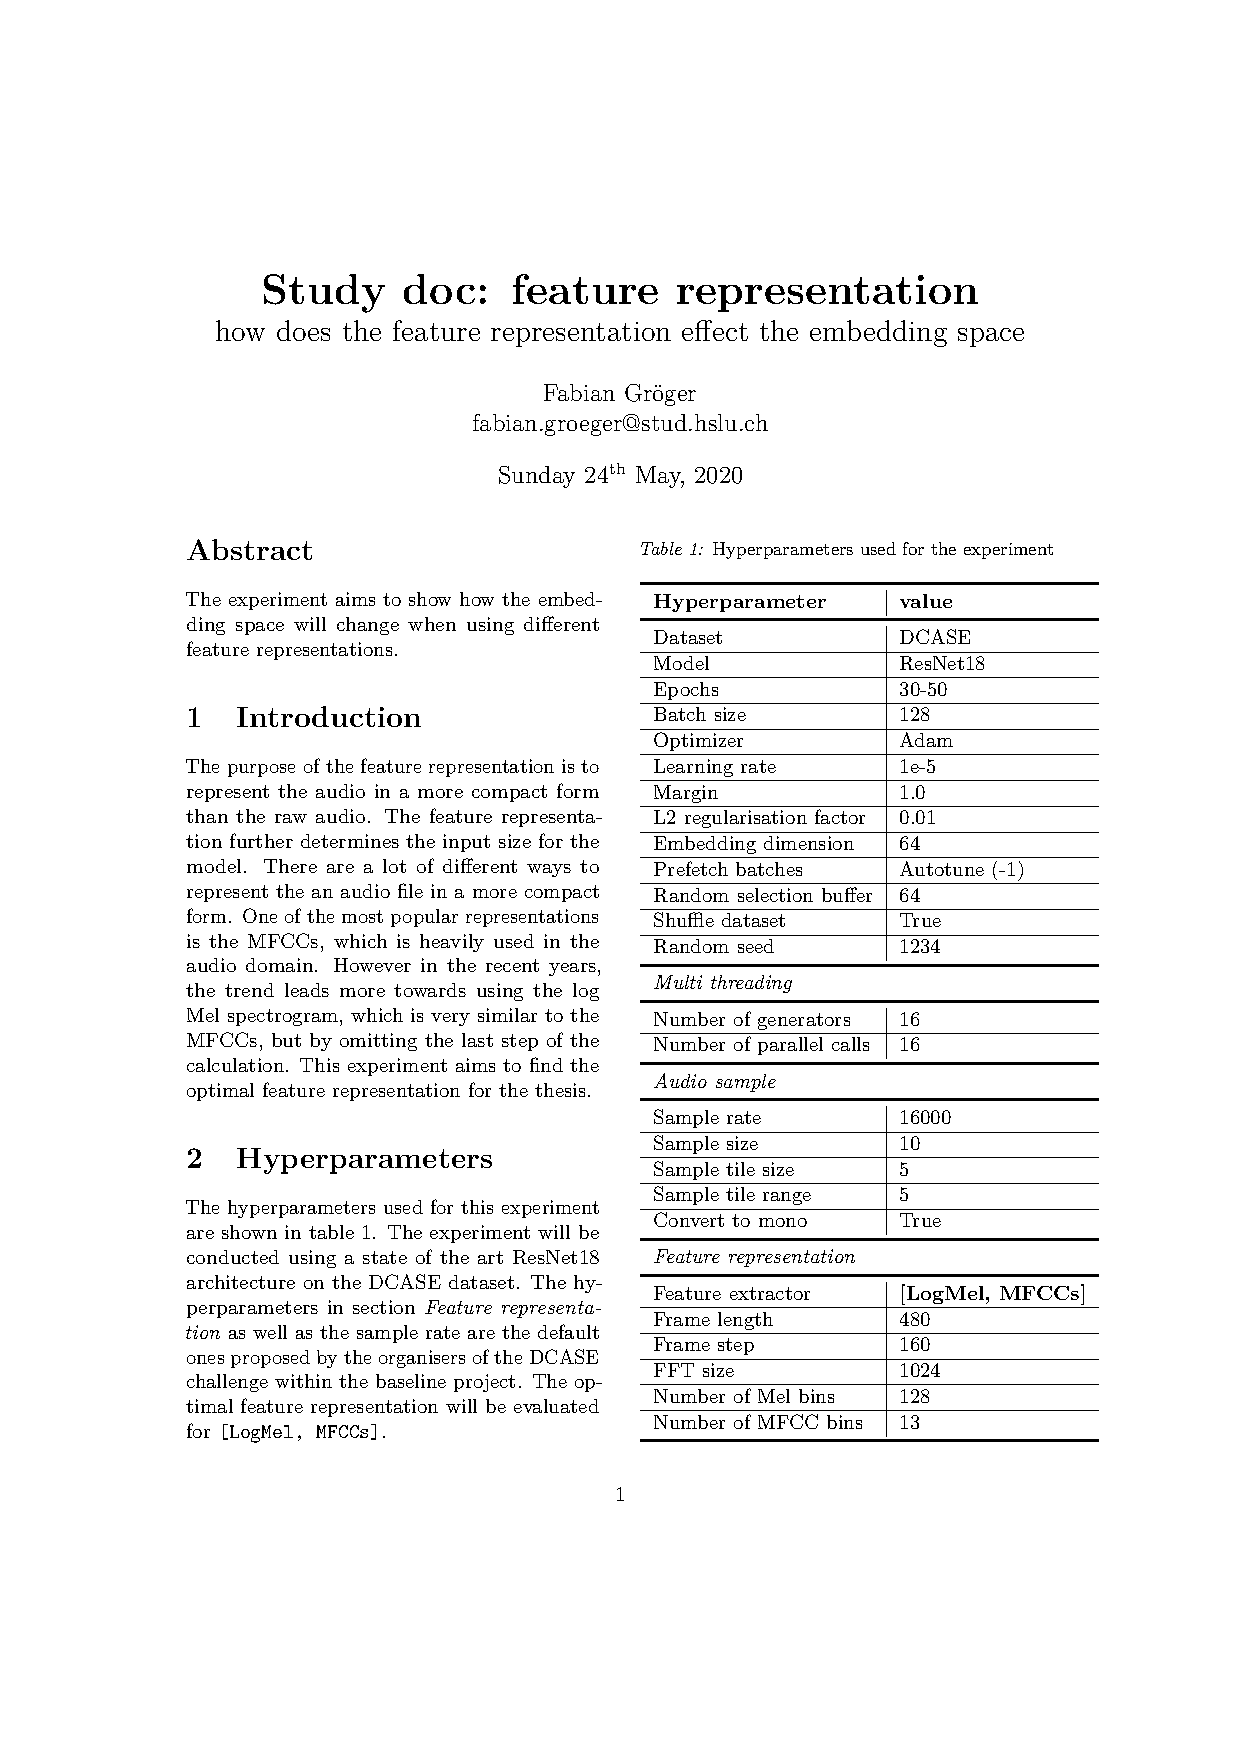
\includepdf[scale=1.0, pages=1-]{study-doc/experiment_feature/Study_Doc_feature_representation.pdf}

\chapter{Qualitative analysis}
\label{app:Qualitative-analysis}

\section{Interview guide}
\label{sec:Interview-Guide}


\includepdf[scale=0.9, pages=1-]{files/bachelor_thesis_interview_guide.pdf}

\section{Interview including answers}
\label{sec:Interview-Answers}


\includepdf[scale=0.9, pages=1-]{files/bachelor_thesis_interview.pdf}

\chapter{Detailed hyperparameters of the models}
\label{app:detailed-hyperparameters}

\begin{table}[ht]
    \centering
    \caption{Detailed hyperparameters of the optimal embedding architecture for the noise detection dataset}
	\label{tab:Hyperparameters-Detailed-DCASE}
    \begin{tabular}{l|l}
        \toprule
        \textbf{Hyperparameter} & \textbf{value} \\ 
        \midrule[1pt]
        Dataset & DCASE \\
        \hline
        Model & ResNet18 \\ 
        \hline
        Epochs & 110 \\ 
        \hline
        Batch size & 64 \\ 
        \hline
        Optimizer & Adam \\ 
        \hline
        Learning rate & 1e-5 \\
        \hline
        Margin & 1.0 \\
        \hline
        L2 regularisation amount & 0.01 \\
        \hline
        Embedding dimension & 256 \\
        \hline
        Prefetch batches & Autotune (-1) \\ 
        \hline
        Random selection buffer & 32 \\ 
        \hline
        Shuffle dataset & True \\
        \hline
        Random seed & 1234 \\
        \midrule[1pt]
        \multicolumn{2}{l}{\textit{Multi threading}} \\
        \midrule[1pt]
        Number of generators & 16 \\ 
        \hline
        Number of parallel calls & 16 \\
        \midrule[1pt]
        \multicolumn{2}{l}{\textit{Audio sample}} \\
        \midrule[1pt]
        Sample rate & 16000 \\ 
        \hline
        Sample size & 10s \\
        \hline
        Sample tile size & 5s \\
        \hline
        Sample tile range & 5s \\
        \hline
        Convert to mono & True \\
        \midrule[1pt]
        \multicolumn{2}{l}{\textit{Feature representation}} \\
        \midrule[1pt]
        Feature extractor & LogMelExtractor \\ 
        \hline
        Frame length & 480 \\
        \hline
        Frame step & 160 \\
        \hline
        FFT size & 1024 \\
        \hline
        Number of Mel bins & 128 \\
        \hline
        Number of MFCC bins & 13 \\
        \bottomrule
    \end{tabular}
\end{table}

\begin{table}[ht]
    \centering
    \caption{Detailed hyperparameters of the optimal embedding architecture for the music dataset}
	\label{tab:Hyperparameters-Detailed-Music}
    \begin{tabular}{l|l}
        \toprule
        \textbf{Hyperparameter} & \textbf{value} \\ 
        \midrule[1pt]
        Dataset & MusicDataset \\
        \hline
        Model & ResNet18 \\ 
        \hline
        Epochs & 130 \\ 
        \hline
        Batch size & 32 \\ 
        \hline
        Optimizer & Adam \\ 
        \hline
        Learning rate & 1e-5 \\
        \hline
        Margin & 1.0 \\
        \hline
        L2 regularisation amount & 0.01 \\
        \hline
        Embedding dimension & 256 \\
        \hline
        Prefetch batches & Autotune (-1) \\ 
        \hline
        Random selection buffer & 16 \\ 
        \hline
        Shuffle dataset & True \\
        \hline
        Random seed & 1234 \\
        \midrule[1pt]
        \multicolumn{2}{l}{\textit{Multi threading}} \\
        \midrule[1pt]
        Number of generators & 16 \\ 
        \hline
        Number of parallel calls & 16 \\
        \midrule[1pt]
        \multicolumn{2}{l}{\textit{Audio sample}} \\
        \midrule[1pt]
        Sample rate & 44100 \\ 
        \hline
        Sample size & variable \\
        \hline
        Sample tile size & 10s \\
        \hline
        Sample tile range & 40s \\
        \hline
        Convert to mono & True \\
        \midrule[1pt]
        \multicolumn{2}{l}{\textit{Feature representation}} \\
        \midrule[1pt]
        Feature extractor & LogMelExtractor \\ 
        \hline
        Frame length & 480 \\
        \hline
        Frame step & 160 \\
        \hline
        FFT size & 1024 \\
        \hline
        Number of Mel bins & 128 \\
        \hline
        Number of MFCC bins & 13 \\
        \bottomrule
    \end{tabular}
\end{table}

\clearpage
\landscapevalues

\chapter{Work journal}
\label{app:Work-Journal}
Within this chapter, the whole work journal of the thesis is shown. The journal is divided into subcategories, so that the \fullref{tab:Work-Journal} is more pleased to read. These categories show what exactly was done in the different project phases, which can be seen in the \fullref{fig:Project-Plan}. There is also one more category called \flqq General\frqq, where all the administrative tasks are shown, including the meetings with the advisor.

\begin{longtable}{| p{.10\textwidth} | p{.20\textwidth} | p{.50\textwidth} | p{.10\textwidth} |} 
	\caption{Work Journal}
	\label{tab:Work-Journal} \\
    \hline
    \textbf{Date} &
    \textbf{Task} &
    \textbf{Details} &
    \textbf{No. hours} \\
    \hline
    \multicolumn{4}{|l|}{\textbf{General}} \\
    \hline
    17.02.2020 & preparation for kick-off meeting & 
        \begin{minipage}{5in}
        \vskip 4pt
        \begin{itemize}
        \setlength\itemsep{0em}
        \item thesis description read carefully again
        \item questions of unclear matters
        \end{itemize}
        \vskip 4pt
        \end{minipage}
        & 1h  \\
    \hline
    17.02.2020 & kick-off meeting (number 1)& 
        \begin{minipage}{5in}
        \vskip 4pt
        \begin{itemize}
        \setlength\itemsep{0em}
        \item discussed different topics which are important for the implementation of the project
        \end{itemize}
        \vskip 4pt
        \end{minipage}
        & 1h 30min  \\
    \hline
    24.02.2020 & meeting (number 2) & 
        \begin{minipage}{5in}
        \vskip 4pt
        \begin{itemize}
        \setlength\itemsep{0em}
        \item preparation of the meeting
        \item meeting itself
        \end{itemize}
        \vskip 4pt
        \end{minipage}
        & 2h  \\
    \hline
    02.03.2020 & meeting (number 3) & 
        \begin{minipage}{5in}
        \vskip 4pt
        \begin{itemize}
        \setlength\itemsep{0em}
        \item preparation of the meeting
        \item meeting itself
        \end{itemize}
        \vskip 4pt
        \end{minipage}
        & 2h  \\
    \hline
    02.03.2020 & meeting GPU with Thomas Koller & 
        \begin{minipage}{5in}
        \vskip 4pt
        \begin{itemize}
        \setlength\itemsep{0em}
        \item preparation of the meeting
        \item meeting itself
        \end{itemize}
        \vskip 4pt
        \end{minipage}
        & 0.5h  \\
    \hline
    09.03.2020 & meeting (number 4) & 
        \begin{minipage}{5in}
        \vskip 4pt
        \begin{itemize}
        \setlength\itemsep{0em}
        \item preparation of the meeting
        \item meeting itself
        \end{itemize}
        \vskip 4pt
        \end{minipage}
        & 2h  \\
    \hline
    16.03.2020 & meeting (number 5) & 
        \begin{minipage}{5in}
        \vskip 4pt
        \begin{itemize}
        \setlength\itemsep{0em}
        \item preparation of the meeting
        \item meeting itself
        \end{itemize}
        \vskip 4pt
        \end{minipage}
        & 2h  \\
    \hline
    23.03.2020 & meeting (number 6) & 
        \begin{minipage}{5in}
        \vskip 4pt
        \begin{itemize}
        \setlength\itemsep{0em}
        \item preparation of the meeting
        \item meeting itself
        \end{itemize}
        \vskip 4pt
        \end{minipage}
        & 2h  \\
    \hline
    30.03.2020 & meeting (number 7) & 
        \begin{minipage}{5in}
        \vskip 4pt
        \begin{itemize}
        \setlength\itemsep{0em}
        \item preparation of the meeting
        \item meeting itself
        \end{itemize}
        \vskip 4pt
        \end{minipage}
        & 2h  \\
    \hline
    06.04.2020 & meeting (number 8) & 
        \begin{minipage}{5in}
        \vskip 4pt
        \begin{itemize}
        \setlength\itemsep{0em}
        \item preparation of the meeting
        \item meeting itself
        \end{itemize}
        \vskip 4pt
        \end{minipage}
        & 2h  \\
    \hline
    15.04.2020 & meeting (number 9) & 
        \begin{minipage}{5in}
        \vskip 4pt
        \begin{itemize}
        \setlength\itemsep{0em}
        \item preparation of the meeting
        \item meeting itself
        \end{itemize}
        \vskip 4pt
        \end{minipage}
        & 2h  \\
    \hline
    20.04.2020 & meeting (number 10) & 
        \begin{minipage}{5in}
        \vskip 4pt
        \begin{itemize}
        \setlength\itemsep{0em}
        \item preparation of the meeting
        \item meeting itself
        \end{itemize}
        \vskip 4pt
        \end{minipage}
        & 2h  \\
    \hline
    21.04.2020 & interim presentation & 
        \begin{minipage}{5in}
        \vskip 4pt
        \begin{itemize}
        \setlength\itemsep{0em}
        \item preparation
        \item presentation
        \item discussion
        \end{itemize}
        \vskip 4pt
        \end{minipage}
        & 5h  \\
    \hline
    27.04.2020 & meeting (number 11) & 
        \begin{minipage}{5in}
        \vskip 4pt
        \begin{itemize}
        \setlength\itemsep{0em}
        \item preparation of the meeting
        \item meeting itself
        \end{itemize}
        \vskip 4pt
        \end{minipage}
        & 2h  \\
    \hline
    04.05.2020 & meeting (number 12) & 
        \begin{minipage}{5in}
        \vskip 4pt
        \begin{itemize}
        \setlength\itemsep{0em}
        \item preparation of the meeting
        \item meeting itself
        \end{itemize}
        \vskip 4pt
        \end{minipage}
        & 2h  \\
    \hline
    11.05.2020 & meeting (number 13) & 
        \begin{minipage}{5in}
        \vskip 4pt
        \begin{itemize}
        \setlength\itemsep{0em}
        \item preparation of the meeting
        \item meeting itself
        \end{itemize}
        \vskip 4pt
        \end{minipage}
        & 2h  \\
    \hline
    19.05.2020 & meeting (number 14) & 
        \begin{minipage}{5in}
        \vskip 4pt
        \begin{itemize}
        \setlength\itemsep{0em}
        \item preparation of the meeting
        \item meeting itself
        \end{itemize}
        \vskip 4pt
        \end{minipage}
        & 2h  \\
    \hline
    25.05.2020 & meeting (number 15) & 
        \begin{minipage}{5in}
        \vskip 4pt
        \begin{itemize}
        \setlength\itemsep{0em}
        \item preparation of the meeting
        \item meeting itself
        \end{itemize}
        \vskip 4pt
        \end{minipage}
        & 2h  \\
    \hline
    28.05.2020 & interview Emanuel Oehri & 
        \begin{minipage}{5in}
        \vskip 4pt
        \begin{itemize}
        \setlength\itemsep{0em}
        \item preparation of interview guide
        \item preparation of resources
        \item interview itself
        \end{itemize}
        \vskip 4pt
        \end{minipage}
        & 6h  \\
    \hline
    \multicolumn{4}{|l|}{\textbf{Documentation}} \\
    \hline
    17.02.2020 & documentation setup & 
        \begin{minipage}{5in}
        \vskip 4pt
        \begin{itemize}
        \setlength\itemsep{0em}
        \item project setup
        \item latex document setup
        \item German transcribed to English
        \item built default documentation structure
        \end{itemize}
        \vskip 4pt
        \end{minipage}
        & 2h  \\
    \hline
    19.02.2020 & dataset documented & 
        \begin{minipage}{5in}
        \vskip 4pt
        \begin{itemize}
        \setlength\itemsep{0em}
        \item SINS database
        \item DCASE task dataset
        \end{itemize}
        \vskip 4pt
        \end{minipage}
        & 3h  \\
    \hline
    24.02.2020 & dataset section finished & 
        \begin{minipage}{5in}
        \vskip 4pt
        \begin{itemize}
        \setlength\itemsep{0em}
        \item created table of the recorded activities in the \gls{SINS} database
        \item reread section and corrected
        \end{itemize}
        \vskip 4pt
        \end{minipage}
        & 1h  \\
    \hline
    02.03.2020 & triplet Loss section finished & 
        \begin{minipage}{5in}
        \vskip 4pt
        \begin{itemize}
        \setlength\itemsep{0em}
        \item documented Triplet Loss in related work
        \item reread section and corrected
        \end{itemize}
        \vskip 4pt
        \end{minipage}
        & 2h  \\
    \hline
    03.03.2020 & Tile2Vec section finished & 
        \begin{minipage}{5in}
        \vskip 4pt
        \begin{itemize}
        \setlength\itemsep{0em}
        \item documented Tile2Vec in related work
        \item reread section and corrected
        \item corrected equations
        \end{itemize}
        \vskip 4pt
        \end{minipage}
        & 2h  \\
    \hline
    05.03.2020 & started with intro to neural networks & 
        \begin{minipage}{5in}
        \vskip 4pt
        \begin{itemize}
        \setlength\itemsep{0em}
        \item researched neural networks
        \item documented neural networks
        \end{itemize}
        \vskip 4pt
        \end{minipage}
        & 4h  \\
    \hline
    06.03.2020 & finished with intro to neural networks & 
        \begin{minipage}{5in}
        \vskip 4pt
        \begin{itemize}
        \setlength\itemsep{0em}
        \item documented neural networks
        \end{itemize}
        \vskip 4pt
        \end{minipage}
        & 4h  \\
    \hline
    05.03.2020 & started with intro to convolutional neural networks & 
        \begin{minipage}{5in}
        \vskip 4pt
        \begin{itemize}
        \setlength\itemsep{0em}
        \item researched convolutional neural networks
        \item documented convolutional neural networks
        \end{itemize}
        \vskip 4pt
        \end{minipage}
        & 2h  \\
    \hline
    09.03.2020 & finished intro to convolutional neural networks & 
        \begin{minipage}{5in}
        \vskip 4pt
        \begin{itemize}
        \setlength\itemsep{0em}
        \item documented convolutional neural networks
        \end{itemize}
        \vskip 4pt
        \end{minipage}
        & 3h  \\
    \hline
    09.03.2020 & documented various parts & 
        \begin{minipage}{5in}
        \vskip 4pt
        \begin{itemize}
        \setlength\itemsep{0em}
        \item documented project plan and milestones
        \item documented introduction
        \item documented appendix
        \item documented into to clustering
        \end{itemize}
        \vskip 4pt
        \end{minipage}
        & 3h  \\
    \hline
    11.03.2020 & document changes applied from meeting & 
        \begin{minipage}{5in}
        \vskip 4pt
        \begin{itemize}
        \setlength\itemsep{0em}
        \item moving Dataset to related work
        \item changed denotation of loss function
        \item changed \gls{NN} section
        \end{itemize}
        \vskip 4pt
        \end{minipage}
        & 1h  \\
    \hline
    11.03.2020 & finished intro to gated recurrent unit & 
        \begin{minipage}{5in}
        \vskip 4pt
        \begin{itemize}
        \setlength\itemsep{0em}
        \item documented gated recurrent unit
        \end{itemize}
        \vskip 4pt
        \end{minipage}
        & 2h  \\
    \hline
    13.03.2020 & finished status in relation to project & 
        \begin{minipage}{5in}
        \vskip 4pt
        \begin{itemize}
        \setlength\itemsep{0em}
        \item researched state-of-the-art in audio deep learning
        \item documented status in relation to project
        \end{itemize}
        \vskip 4pt
        \end{minipage}
        & 4h  \\
    \hline
    15.03.2020 & finished related work & 
        \begin{minipage}{5in}
        \vskip 4pt
        \begin{itemize}
        \setlength\itemsep{0em}
        \item researched dilated convolution
        \item documented dilated convolution
        \end{itemize}
        \vskip 4pt
        \end{minipage}
        & 2h  \\
    \hline
    15.03.2020 & milestone review & 
        \begin{minipage}{5in}
        \vskip 4pt
        \begin{itemize}
        \setlength\itemsep{0em}
        \item M1 milestone review
        \end{itemize}
        \vskip 4pt
        \end{minipage}
        & 1h  \\
    \hline
    27.03.2020 & started with changes from Daniel & 
        \begin{minipage}{5in}
        \vskip 4pt
        \begin{itemize}
        \setlength\itemsep{0em}
        \item related work changes
        \end{itemize}
        \vskip 4pt
        \end{minipage}
        & 2h  \\
    \hline
    28.03.2020 & started with chapter 3, ideas and concepts & 
        \begin{minipage}{5in}
        \vskip 4pt
        \begin{itemize}
        \setlength\itemsep{0em}
        \item data preprocessing
        \item feature extraction
        \item data augmentation
        \end{itemize}
        \vskip 4pt
        \end{minipage}
        & 3h  \\
    \hline
    29.03.2020 & milestone review & 
        \begin{minipage}{5in}
        \vskip 4pt
        \begin{itemize}
        \setlength\itemsep{0em}
        \item M2 milestone review
        \end{itemize}
        \vskip 4pt
        \end{minipage}
        & 1h  \\
    \hline
    06.04.2020 & finished with changes from Daniel & 
        \begin{minipage}{5in}
        \vskip 4pt
        \begin{itemize}
        \setlength\itemsep{0em}
        \item related Work changes
        \end{itemize}
        \vskip 4pt
        \end{minipage}
        & 1h  \\
    \hline
    06.04.2020 & worked on chapter 3, ideas and concepts & 
        \begin{minipage}{5in}
        \vskip 4pt
        \begin{itemize}
        \setlength\itemsep{0em}
        \item input pipeline
        \item triplet selection
        \item refactoring of chapter
        \end{itemize}
        \vskip 4pt
        \end{minipage}
        & 3h 30min  \\
    \hline
    12.04.2020 & milestone review & 
        \begin{minipage}{5in}
        \vskip 4pt
        \begin{itemize}
        \setlength\itemsep{0em}
        \item M3 milestone review
        \end{itemize}
        \vskip 4pt
        \end{minipage}
        & 1h  \\
    \hline
    13.04.2020 & worked on chapter 3, ideas and concepts & 
        \begin{minipage}{5in}
        \vskip 4pt
        \begin{itemize}
        \setlength\itemsep{0em}
        \item rewrote most of the sections
        \item finished draft of chapter 3
        \end{itemize}
        \vskip 4pt
        \end{minipage}
        & 3h \\
    \hline
    13.04.2020 & worked on chapter 4, method &
        \begin{minipage}{5in}
        \vskip 4pt
        \begin{itemize}
        \setlength\itemsep{0em}
        \item updated project plan
        \item started with documentation of procedure model
        \end{itemize}
        \vskip 4pt
        \end{minipage}
        & 1h \\
    \hline
    15.04.2020 & worked on interim presentation &
        \begin{minipage}{5in}
        \vskip 4pt
        \begin{itemize}
        \setlength\itemsep{0em}
        \item created slides
        \item reviewed slides
        \end{itemize}
        \vskip 4pt
        \end{minipage}
        & 4h \\
    \hline
    16.04.2020 & worked on interim presentation &
        \begin{minipage}{5in}
        \vskip 4pt
        \begin{itemize}
        \setlength\itemsep{0em}
        \item practised presentation
        \end{itemize}
        \vskip 4pt
        \end{minipage}
        & 4h \\
    \hline
    20.04.2020 & worked on interim presentation &
        \begin{minipage}{5in}
        \vskip 4pt
        \begin{itemize}
        \setlength\itemsep{0em}
        \item practised presentation
        \end{itemize}
        \vskip 4pt
        \end{minipage}
        & 2h \\
    \hline
    24.04.2020 & worked on chapter 4, method &
        \begin{minipage}{5in}
        \vskip 4pt
        \begin{itemize}
        \setlength\itemsep{0em}
        \item project structure
        \item resources
        \item evaluation
        \end{itemize}
        \vskip 4pt
        \end{minipage}
        & 6h \\
    \hline
    25.04.2020 & worked on chapter 5, realisation &
        \begin{minipage}{5in}
        \vskip 4pt
        \begin{itemize}
        \setlength\itemsep{0em}
        \item overall structure
        \item started with UML diagrams
        \end{itemize}
        \vskip 4pt
        \end{minipage}
        & 3h \\
    \hline
    30.04.2020 & thesis changes of chapter 1, 3, 4 and 5 &
        \begin{minipage}{5in}
        \vskip 4pt
        \begin{itemize}
        \setlength\itemsep{0em}
        \item thesis corrections
        \end{itemize}
        \vskip 4pt
        \end{minipage}
        & 4h \\
    \hline
    03.05.2020 & milestone review & 
        \begin{minipage}{5in}
        \vskip 4pt
        \begin{itemize}
        \setlength\itemsep{0em}
        \item M5 milestone review
        \end{itemize}
        \vskip 4pt
        \end{minipage}
        & 1h  \\
    \hline
    06.05.2020 & worked on chapter 5, realisation &
        \begin{minipage}{5in}
        \vskip 4pt
        \begin{itemize}
        \setlength\itemsep{0em}
        \item documented realisation
        \item created UML diagrams
        \end{itemize}
        \vskip 4pt
        \end{minipage}
        & 4h \\
    \hline
    08.05.2020 & worked on chapter 5, realisation &
        \begin{minipage}{5in}
        \vskip 4pt
        \begin{itemize}
        \setlength\itemsep{0em}
        \item finished with realisation
        \end{itemize}
        \vskip 4pt
        \end{minipage}
        & 6h \\
    \hline
    23.05.2020 & worked on chapter 6, results &
        \begin{minipage}{5in}
        \vskip 4pt
        \begin{itemize}
        \setlength\itemsep{0em}
        \item started with results from DCASE challenge dataset
        \end{itemize}
        \vskip 4pt
        \end{minipage}
        & 4h \\
    \hline
    25.05.2020 & worked on chapter 4, method &
        \begin{minipage}{5in}
        \vskip 4pt
        \begin{itemize}
        \setlength\itemsep{0em}
        \item added detailed information about work packages, artefacts and phases
        \item added risk analysis
        \end{itemize}
        \vskip 4pt
        \end{minipage}
        & 3h \\
    \hline
    30.05.2020 & worked on chapter 6, results &
        \begin{minipage}{5in}
        \vskip 4pt
        \begin{itemize}
        \setlength\itemsep{0em}
        \item results from DCASE challenge dataset
        \item results from music dataset
        \end{itemize}
        \vskip 4pt
        \end{minipage}
        & 6h \\
    \hline
    31.05.2020 & worked on chapter 6, results &
        \begin{minipage}{5in}
        \vskip 4pt
        \begin{itemize}
        \setlength\itemsep{0em}
        \item finished with chapter
        \end{itemize}
        \vskip 4pt
        \end{minipage}
        & 3h \\
    \hline
    31.05.2020 & worked on chapter 7, conclusion &
        \begin{minipage}{5in}
        \vskip 4pt
        \begin{itemize}
        \setlength\itemsep{0em}
        \item project conclusion
        \item discussion
        \item outlook
        \end{itemize}
        \vskip 4pt
        \end{minipage}
        & 5h \\
    \hline
    01.06.2020 & thesis corrections &
        \begin{minipage}{5in}
        \vskip 4pt
        \begin{itemize}
        \setlength\itemsep{0em}
        \item corrections
        \end{itemize}
        \vskip 4pt
        \end{minipage}
        & 4h \\
    \hline
    02.06.2020 & thesis corrections &
        \begin{minipage}{5in}
        \vskip 4pt
        \begin{itemize}
        \setlength\itemsep{0em}
        \item corrections
        \end{itemize}
        \vskip 4pt
        \end{minipage}
        & 5h \\
    \hline
    \multicolumn{4}{|l|}{\textbf{Research}} \\
    \hline
    17.02.2020 & research dataset & 
        \begin{minipage}{5in}
        \vskip 4pt
        \begin{itemize}
        \setlength\itemsep{0em}
        \item finished with DCASE - challenge description
        \item started with SINS database paper
        \end{itemize}
        \vskip 4pt
        \end{minipage}
        & 2h 30min  \\
    \hline
    21.02.2020 & audio processing research & 
        \begin{minipage}{5in}
        \vskip 4pt
        \begin{itemize}
        \setlength\itemsep{0em}
        \item \gls{FT}
        \item \gls{FFT}
        \item \gls{DFT}
        \item Spectrogram
        \item started with related work documentation
        \end{itemize}
        \vskip 4pt
        \end{minipage}
        & 5h  \\
    \hline
    26.02.2020 & audio processing research & 
        \begin{minipage}{5in}
        \vskip 4pt
        \begin{itemize}
        \setlength\itemsep{0em}
        \item \gls{MFCC}
        \item documenting research in related work
        \end{itemize}
        \vskip 4pt
        \end{minipage}
        & 3h  \\
    \hline
    27.02.2020 & audio processing research & 
        \begin{minipage}{5in}
        \vskip 4pt
        \begin{itemize}
        \setlength\itemsep{0em}
        \item \gls{MFCC}
        \item finished documenting research in related work
        \end{itemize}
        \vskip 4pt
        \end{minipage}
        & 4h  \\
    \hline
    28.02.2020 & triplet loss research & 
        \begin{minipage}{5in}
        \vskip 4pt
        \begin{itemize}
        \setlength\itemsep{0em}
        \item read various paper on triplet loss
        \end{itemize}
        \vskip 4pt
        \end{minipage}
        & 3h  \\
    \hline
    01.03.2020 & triplet loss research & 
        \begin{minipage}{5in}
        \vskip 4pt
        \begin{itemize}
        \setlength\itemsep{0em}
        \item current research on triplet loss with audio
        \end{itemize}
        \vskip 4pt
        \end{minipage}
        & 2h  \\
    \hline
    02.03.2020 & Tile2Vec research & 
        \begin{minipage}{5in}
        \vskip 4pt
        \begin{itemize}
        \setlength\itemsep{0em}
        \item read various paper on tile2vec
        \item started documenting tile2vec in related work
        \end{itemize}
        \vskip 4pt
        \end{minipage}
        & 5h  \\
    \hline
    31.05.2020 & documented other relevant work & 
        \begin{minipage}{5in}
        \vskip 4pt
        \begin{itemize}
        \setlength\itemsep{0em}
        \item summarised other relevant work for the thesis
        \end{itemize}
        \vskip 4pt
        \end{minipage}
        & 2h  \\
    \hline
    \multicolumn{4}{|l|}{\textbf{Realisation}} \\
    \hline
    14.03.2020 & started with project setup and input pipeline & 
        \begin{minipage}{5in}
        \vskip 4pt
        \begin{itemize}
        \setlength\itemsep{0em}
        \item set up the GitHub project
        \item started with input pipeline
        \item generator of triplets
        \end{itemize}
        \vskip 4pt
        \end{minipage}
        & 8h  \\
    \hline
    15.03.2020 & started with input pipeline & 
        \begin{minipage}{5in}
        \vskip 4pt
        \begin{itemize}
        \setlength\itemsep{0em}
        \item first test cases for input pipeline
        \item implemented first idea of similarity measure between audios
        \end{itemize}
        \vskip 4pt
        \end{minipage}
        & 2h  \\
    \hline
    16.03.2020 & input pipeline finished & 
        \begin{minipage}{5in}
        \vskip 4pt
        \begin{itemize}
        \setlength\itemsep{0em}
        \item finished input pipeline
        \item finished unit test for pipeline
        \end{itemize}
        \vskip 4pt
        \end{minipage}
        & 7h  \\
    \hline
    18.03.2020 & project setup & 
        \begin{minipage}{5in}
        \vskip 4pt
        \begin{itemize}
        \setlength\itemsep{0em}
        \item finished project structure
        \end{itemize}
        \vskip 4pt
        \end{minipage}
        & 2h  \\
    \hline
    18.03.2020 & implementation & 
        \begin{minipage}{5in}
        \vskip 4pt
        \begin{itemize}
        \setlength\itemsep{0em}
        \item triplet loss implemented
        \item dense model implemented
        \item started with projector visualisation
        \end{itemize}
        \vskip 4pt
        \end{minipage}
        & 5h  \\
    \hline
    20.03.2020 & implementation & 
        \begin{minipage}{5in}
        \vskip 4pt
        \begin{itemize}
        \setlength\itemsep{0em}
        \item train workflow implemented
        \end{itemize}
        \vskip 4pt
        \end{minipage}
        & 5h  \\
    \hline
    23.03.2020 & implementation & 
        \begin{minipage}{5in}
        \vskip 4pt
        \begin{itemize}
        \setlength\itemsep{0em}
        \item tested models and workflow on GPU
        \item convolutional model implemented
        \end{itemize}
        \vskip 4pt
        \end{minipage}
        & 5h  \\
    \hline
    25.03.2020 & implementation & 
        \begin{minipage}{5in}
        \vskip 4pt
        \begin{itemize}
        \setlength\itemsep{0em}
        \item convolutional model edited (1D and 2D)
        \item training workflow edited
        \end{itemize}
        \vskip 4pt
        \end{minipage}
        & 4h  \\
    \hline
    27.03.2020 & implementation & 
        \begin{minipage}{5in}
        \vskip 4pt
        \begin{itemize}
        \setlength\itemsep{0em}
        \item factories implemented
        \item metrics implemented
        \end{itemize}
        \vskip 4pt
        \end{minipage}
        & 5h  \\
    \hline
    31.03.2020 & implementation & 
        \begin{minipage}{5in}
        \vskip 4pt
        \begin{itemize}
        \setlength\itemsep{0em}
        \item GRU Model implemented
        \item refactoring
        \end{itemize}
        \vskip 4pt
        \end{minipage}
        & 4h  \\
    \hline
    03.04.2020 & implementation & 
        \begin{minipage}{5in}
        \vskip 4pt
        \begin{itemize}
        \setlength\itemsep{0em}
        \item music dataset pipeline
        \item unit tests finished
        \item documentation of code
        \item worked on classifier
        \end{itemize}
        \vskip 4pt
        \end{minipage}
        & 6h  \\
    \hline
    04.04.2020 & implementation & 
        \begin{minipage}{5in}
        \vskip 4pt
        \begin{itemize}
        \setlength\itemsep{0em}
        \item worked on evaluation workflow
        \end{itemize}
        \vskip 4pt
        \end{minipage}
        & 3h  \\
    \hline
    07.04.2020 & implementation & 
        \begin{minipage}{5in}
        \vskip 4pt
        \begin{itemize}
        \setlength\itemsep{0em}
        \item input pipeline multiprocessing
        \end{itemize}
        \vskip 4pt
        \end{minipage}
        & 5h  \\
    \hline
    08.04.2020 & implementation & 
        \begin{minipage}{5in}
        \vskip 4pt
        \begin{itemize}
        \setlength\itemsep{0em}
        \item changed triplet selection of datasets
        \end{itemize}
        \vskip 4pt
        \end{minipage}
        & 6h  \\
    \hline
    12.04.2020 & implementation & 
        \begin{minipage}{5in}
        \vskip 4pt
        \begin{itemize}
        \setlength\itemsep{0em}
        \item finished evaluation workflow
        \item added new metrics to classifier
        \end{itemize}
        \vskip 4pt
        \end{minipage}
        & 4h  \\
    \hline
    14.04.2020 & implementation & 
        \begin{minipage}{5in}
        \vskip 4pt
        \begin{itemize}
        \setlength\itemsep{0em}
        \item input pipeline speedup
        \end{itemize}
        \vskip 4pt
        \end{minipage}
        & 3h  \\
    \hline
    15.04.2020 & implementation & 
        \begin{minipage}{5in}
        \vskip 4pt
        \begin{itemize}
        \setlength\itemsep{0em}
        \item added ResNet architecture
        \end{itemize}
        \vskip 4pt
        \end{minipage}
        & 4h  \\
    \hline
    22.04.2020 & implementation & 
        \begin{minipage}{5in}
        \vskip 4pt
        \begin{itemize}
        \setlength\itemsep{0em}
        \item bug fixes
        \item added zero filtering triplet loss strategy
        \end{itemize}
        \vskip 4pt
        \end{minipage}
        & 4h  \\
    \hline
    28.04.2020 & implementation & 
        \begin{minipage}{5in}
        \vskip 4pt
        \begin{itemize}
        \setlength\itemsep{0em}
        \item regularisation added to models
        \end{itemize}
        \vskip 4pt
        \end{minipage}
        & 4h  \\
    \hline
    30.04.2020 & implementation & 
        \begin{minipage}{5in}
        \vskip 4pt
        \begin{itemize}
        \setlength\itemsep{0em}
        \item bug fixes classifier
        \item bug fixes metrics
        \end{itemize}
        \vskip 4pt
        \end{minipage}
        & 3h  \\
    \hline
    05.05.2020 & implementation & 
        \begin{minipage}{5in}
        \vskip 4pt
        \begin{itemize}
        \setlength\itemsep{0em}
        \item added logistic classifier
        \end{itemize}
        \vskip 4pt
        \end{minipage}
        & 1h  \\
    \hline
    08.05.2020 & implementation & 
        \begin{minipage}{5in}
        \vskip 4pt
        \begin{itemize}
        \setlength\itemsep{0em}
        \item big refactoring
        \item code documentation
        \end{itemize}
        \vskip 4pt
        \end{minipage}
        & 4h  \\
    \hline
    \multicolumn{4}{|l|}{\textbf{Experiments}} \\
    \hline
    17.04.2020 until 22.04.2020 & experiment margin & 
        \begin{minipage}{5in}
        \vskip 4pt
        \begin{itemize}
        \setlength\itemsep{0em}
        \item started experiment
        \item evaluated results
        \item created study doc template
        \item wrote study doc
        \end{itemize}
        \vskip 4pt
        \end{minipage}
        & 8h  \\
    \hline
    22.04.2020 until 28.04.2020 & experiment feature & 
        \begin{minipage}{5in}
        \vskip 4pt
        \begin{itemize}
        \setlength\itemsep{0em}
        \item started experiment
        \item evaluated results
        \item wrote study doc
        \end{itemize}
        \vskip 4pt
        \end{minipage}
        & 6h  \\
    \hline
    30.04.2020 until 05.05.2020 & experiment tile size & 
        \begin{minipage}{5in}
        \vskip 4pt
        \begin{itemize}
        \setlength\itemsep{0em}
        \item started experiment
        \item evaluated results
        \item wrote study doc
        \end{itemize}
        \vskip 4pt
        \end{minipage}
        & 6h  \\
    \hline
    06.05.2020 until 11.05.2020 & experiment embedding size & 
        \begin{minipage}{5in}
        \vskip 4pt
        \begin{itemize}
        \setlength\itemsep{0em}
        \item started experiment
        \item evaluated results
        \item wrote study doc
        \end{itemize}
        \vskip 4pt
        \end{minipage}
        & 8h  \\
    \hline
    11.05.2020 until 13.05.2020 & experiment regularisation factor & 
        \begin{minipage}{5in}
        \vskip 4pt
        \begin{itemize}
        \setlength\itemsep{0em}
        \item started experiment
        \item evaluated results
        \item wrote study doc
        \end{itemize}
        \vskip 4pt
        \end{minipage}
        & 5h  \\
    \hline
    15.05.2020 until 20.05.2020 & experiment embedding size larger & 
        \begin{minipage}{5in}
        \vskip 4pt
        \begin{itemize}
        \setlength\itemsep{0em}
        \item started experiment
        \item evaluated results
        \item wrote study doc
        \end{itemize}
        \vskip 4pt
        \end{minipage}
        & 6h  \\
    \hline
    20.05.2020 until 24.05.2020 & final model for DCASE dataset trained & 
        \begin{minipage}{5in}
        \vskip 4pt
        \begin{itemize}
        \setlength\itemsep{0em}
        \item final model trained
        \item evaluated results
        \end{itemize}
        \vskip 4pt
        \end{minipage}
        & 3h  \\
    \hline
    23.05.2020 until 30.05.2020 & final model for music dataset trained & 
        \begin{minipage}{5in}
        \vskip 4pt
        \begin{itemize}
        \setlength\itemsep{0em}
        \item trained model using the same hyperparameters on the music dataset
        \item evaluated results
        \end{itemize}
        \vskip 4pt
        \end{minipage}
        & 5h  \\
    \hline
\end{longtable}

\clearpage
\defaultpagestyle

\chapter{Task definition bachelor thesis}
\label{app:Task-Definition}
Within this chapter the final task definition, which was submitted and accepted by the Transfer Office of the Lucerne University of Applied Sciences and Arts on the 25.02.2020, is attached.

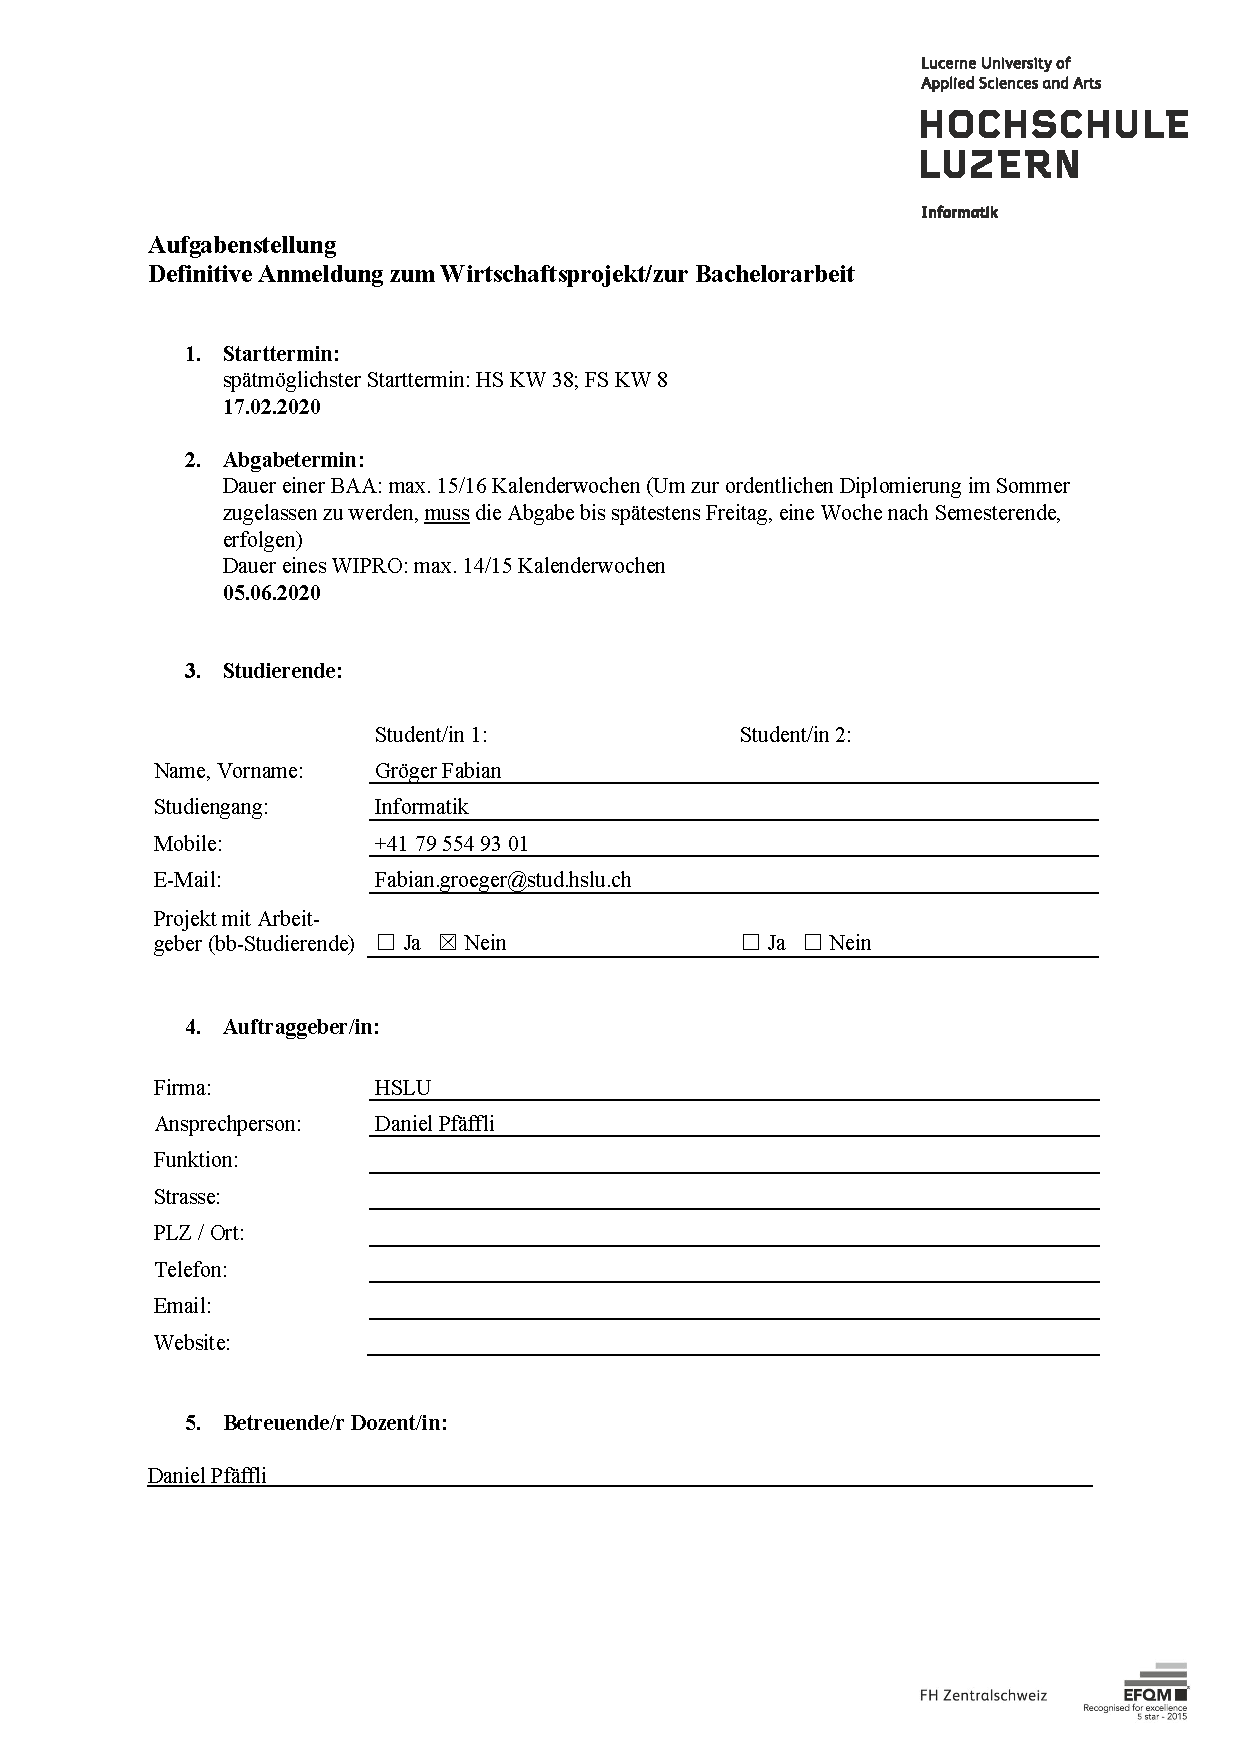
\includepdf[scale=1.0, pages=1-]{files/Aufgabenstellung_DeepEmbeddedMusic.pdf}
